\documentclass[%
    a1paper,%
    17pt,%
    portait,%
    margin=0mm,%
    innermargin=5mm,%
    blockverticalspace=5mm,%
    colspace=5mm,%
    subcolspace=2mm%
]{tikzposter}

\usetitlestyle[]{Wave}

\usepackage[utf8]{inputenc}
\usepackage[T1]{fontenc}

\usepackage[french, english]{babel} % Last language is main language

\usepackage{lmodern} % Latin Modern Font
\usepackage{gensymb} % Generic symbols for both text and math mode

\usepackage{standalone} % Used to generate standalone Tikz

\usepackage{amsmath}   % Main math Package
\usepackage{mathtools} % Extension package to amsmath
\usepackage{amsthm}    % Typesetting theorems (AMS style)
\usepackage{amsfonts}  % More fonts from the AMS
\usepackage{textcomp}  % provide many text symbols
\usepackage{steinmetz} % For phase symbol

\usepackage{xstring}  % Utils to manipulate strings
\usepackage{etoolbox} % Add basic if/then
\usepackage{esvect}   % Beautyfull vectors
\usepackage{graphicx} % Enhanced support for graphics
\usepackage{grffile}  % Used by matlab2tikz

\usepackage{microtype} % typographic tuning
\usepackage{setspace}  % for line spacing, e.g. \onehalfspacing
\usepackage{tabularx}  % table features
\usepackage{enumitem}  % for simple list modifications
\usepackage{booktabs}  % better table support

\usepackage{stackengine} %

\usepackage[load-configurations=abbreviations]{siunitx} % SI units
\sisetup{
    locale = US,
    detect-all,
    range-phrase=--,
    range-units=single
}

\usepackage{tikz}       % Tikz
\usepackage{tikzscale}  % Used to scale Tikz graphics
\usepackage{adjustbox}  % Used to proper positioning of tikz pictures
\usepackage{circuitikz} % Draw electronic circuits
\usepackage{pgfpages}   % Needed to use notes
\usepackage{pgfplots}   % Used to plot functions

\usetikzlibrary{arrows}                   % Arrow tip library
\usetikzlibrary{arrows.meta}              % Add some arrows
\usetikzlibrary{calc}                     % The library allows advanced Coordinate Calculations
\usetikzlibrary{intersections}            % calculate intersections of paths
\usetikzlibrary{matrix}                   %
\usetikzlibrary{patterns}                 %
\usetikzlibrary{shapes}                   % Defines circle and rectangle
\usetikzlibrary{shapes.geometric}         % Use for the shape diamond and isosceles triangle
\usetikzlibrary{snakes}                   % snake=coil and snake=zigzag using segment amplitude=10pt
\usetikzlibrary{positioning}              % Additional options for placing nodes
\usetikzlibrary{3d}                       % Plot 3D shapes
\usetikzlibrary{spy}                      % Creating a magnified area
\usetikzlibrary{decorations.text}         % Used to make text follows a curve
\usetikzlibrary{decorations.pathmorphing} % deformation of a path
\usetikzlibrary{decorations.markings}     % Used for spring and damper
\usetikzlibrary{babel}                    % A tiny library that make the interaction with the babel package easier
\usetikzlibrary{plotmarks}                % This library defines a number of plot marks
\usetikzlibrary{fit}                      % Used to make rectangle as nodes by specifying two points
\usetikzlibrary{backgrounds}              % Used to put things under others

\usepgfplotslibrary{patchplots}
\usepgfplotslibrary{groupplots}

\pgfplotsset{compat=newest}
\pgfplotsset{plot coordinates/math parser=false}

\newlength{\fheight}
\newlength{\fwidth}

\setlength{\fwidth}{85mm}
\setlength{\fheight}{112mm}

\tikzset{>=Stealth}
% Setup default Linewidth
\tikzset{every path/.style={line width=1pt}}

\usepackage{xcolor}% Color extension

\definecolor{mycolor1}{RGB}{79,115,193}
\definecolor{mycolor2}{RGB}{213,91,53}
\definecolor{mycolor3}{RGB}{152,126,49}

\tikzset{%
  block/.style n args={2}{%
    draw,
    fill=white,
    minimum width  = #1,
    minimum height = #2,
  },
  block/.default={1.2cm}{1.0cm}
}

\tikzstyle{branch}=[fill,shape=circle,minimum size=4pt,inner sep=0pt]
\tikzstyle{->top}=[-{Stealth[color=black, scale=0.8]}, draw=white, double=black, double distance=1pt, line width=1pt]
\tikzstyle{<-top}=[{stealth[color=black, scale=0.8]}-, draw=white, double=black, double distance=1pt, line width=1pt]

\tikzstyle{handwriten}=[decorate,decoration={random steps,amplitude=0.1pt,segment length=0.8pt}]

\tikzset{%
  DAC/.style={%
    draw,
    signal,
  }
}

\tikzset{%
  ADC/.style={%
    draw,
    signal,
    signal to = west,
  }
}

\tikzset{%
  gain right/.style={%
    draw,
    regular polygon,
    regular polygon sides = 3,
    inner sep = 2pt,
    shape border rotate=-90
  },
  gain left/.style={%
    draw,
    regular polygon,
    regular polygon sides = 3,
    inner sep = 2pt,
    shape border rotate=90
  },
  gain top/.style={%
    draw,
    regular polygon,
    regular polygon sides = 3,
    inner sep = 2pt,
    shape border rotate=0
  },
  gain bottom/.style={%
    draw,
    regular polygon,
    regular polygon sides = 3,
    inner sep = 2pt,
    shape border rotate=180
  },
}

\tikzset{% Add block with Circled operations
  addc/.style n args={5}{%
    draw,
    fill=white,
    circle,
    outer sep = 0pt,
    inner sep = 0pt,
    minimum size = 2em,
    execute at begin node={\LARGE $#1$},
    append after command={\pgfextra{\let\mainnode=\tikzlastnode}
      \ifx#2\empty\else
      node[draw, circle, outer sep=6pt, inner sep=0pt, above left] at (\mainnode.west) {$#2$}%
      \fi
      \ifx#3\empty\else
      node[draw, circle, outer sep=6pt, inner sep=0pt, above right] at (\mainnode.north) {$#3$}%
      \fi
      \ifx#4\empty\else
      node[draw, circle, outer sep=6pt, inner sep=0pt, below right] at (\mainnode.east) {$#4$}%
      \fi
      \ifx#5\empty\else
      node[draw, circle, outer sep=6pt, inner sep=0pt, below left] at (\mainnode.south) {$#5$}%
      \fi
      }
  },
  addc/.default={+}{}{}{}{},
}

\tikzset{% Add Block
  addb/.style n args={5}{%
    draw,
    fill=white,
    circle,
    outer sep = 0pt,
    inner sep = 0pt,
    minimum size = 2em,
    execute at begin node={\LARGE $#1$},
    append after command={\pgfextra{\let\mainnode=\tikzlastnode}
      \ifx#2\empty\else
      node[outer sep=2pt, inner sep=0pt, above left] at (\mainnode.west) {$#2$}%
      \fi
      \ifx#3\empty\else
      node[outer sep=2pt, inner sep=0pt, above right] at (\mainnode.north) {$#3$}%
      \fi
      \ifx#4\empty\else
      node[outer sep=2pt, inner sep=0pt, below right] at (\mainnode.east) {$#4$}%
      \fi
      \ifx#5\empty\else
      node[outer sep=2pt, inner sep=0pt, below left] at (\mainnode.south) {$#5$}%
      \fi
      }
  },
  addb/.default={+}{}{}{}{},
}

\pgfplotsset{
  every axis plot/.append style={line join=round},
  every axis plot/.append style={line cap=round},
}

\pgfplotsset{grid style={black}}
\pgfplotsset{major grid style={black!30!white}}
\pgfplotsset{minor grid style={black!10!white}}
\pgfplotsset{xmajorgrids}
\pgfplotsset{ymajorgrids}

\pgfplotsset{separate axis lines=false} % draw axis as rectangle and not as 4 lines
\pgfplotsset{every outer x axis line/.append style={black}}
\pgfplotsset{every outer y axis line/.append style={black}}
\pgfplotsset{axis background/.style={fill=white}}
\pgfplotsset{axis x line*=bottom} % solid line on the bottom with thin on the top
\pgfplotsset{axis y line*=left} % solid line on the left with thin on the right

\pgfplotsset{every y tick label/.append style={font=\color{black}}}
\pgfplotsset{every y tick/.append style={black}}
\pgfplotsset{every x tick label/.append style={font=\color{black}}}
\pgfplotsset{every x tick/.append style={black}}

\pgfplotsset{scale only axis=true}

\pgfplotsset{ylabel absolute}

% https://tex.stackexchange.com/questions/54794/using-a-pgfplots-style-legend-in-a-plain-old-tikzpicture#54834

% argument #1: any options
\newenvironment{customlegend}[1][]{%
  \begingroup
  % inits/clears the lists (which might be populated from previous
  % axes):
  \csname pgfplots@init@cleared@structures\endcsname
  \pgfplotsset{#1}%
}{%
  % draws the legend:
  \csname pgfplots@createlegend\endcsname
  \endgroup
}%

% makes \addlegendimage available (typically only available within an
% axis environment):
\def\addlegendimage{\csname pgfplots@addlegendimage\endcsname}

% definition to insert numbers
% \pgfkeys{/pgfplots/number in legend/.style={%
%     /pgfplots/legend image code/.code={%
%       \node at (0.125,-0.0225){#1}; % <= changed x value
%     },%
%   },
% }
\pgfplotsset{
  every legend to name picture/.style={west}
}

\tikzset{%
  spring/.style={%
    thick,
    decoration={
      zigzag,
      pre length  = #1cm,
      post length = #1cm,
      segment length = 6
    },
    decorate
  },
  spring/.default={0.2}
}

\tikzset{%
  coil/.style n args={2}{%
    thick,
    decoration={
      coil,
      pre length  = #1cm,
      post length = #2cm,
      segment length = 4
    },
    decorate
  },
  coil/.default={0.3}{0.3}
}

\tikzset{%
  damper/.style n args={2}{%
    thick,
    decoration={markings, mark connection node=dmp, mark=at position 0.5 with {
        \node (dmp) [thick,
                     inner sep = 0pt,
                     transform shape,
                     rotate  =-90,
                     minimum width  = #1pt,
                     minimum height = #2pt,
                     draw=none] {};
        \draw [thick] ($(dmp.north east)+(0.6*#2pt,0)$) -- (dmp.south east) -- (dmp.south west) -- ($(dmp.north west)+(0.6*#2pt,0)$);
        \draw [thick] ($(dmp.north)+(0,-0.3*#1pt)$) -- ($(dmp.north)+(0,0.3*#1pt)$);
      }
    },
    decorate
  },
  damper/.default={12}{3}
}

\tikzset{%
  actuator/.style n args={2}{%
    thick,
    draw=none,
    decoration={
      markings,
      mark connection node=my node,
      mark=at position .5 with {
        \node [draw, inner sep=0pt, minimum width=#1cm, minimum height=#2cm,
        transform shape, fill=white] (my node) {};
      },
      mark=at position .0 with {
        \draw[<-] (0, 0) -- (my node);
      },
      mark=at position 1.0 with {
        \draw[<-] (0, 0) -- (my node);
      }
    },
    decorate
  },
  actuator/.default={0.5}{0.2}
}

\tikzset{%
  ground/.style n args={2}{%
    fill,
    pattern = north east lines,
    draw = none,
    anchor = north,
    minimum width  = #1cm,
    minimum height = #2cm,
    append after command={
      (\tikzlastnode.north west) edge (\tikzlastnode.north east)
    }
  },
  ground/.default={2.5}{0.3}
}

\tikzset{%
  forcesensor/.style n args={2}{%
    rectangle,
    outer sep=0pt,
    inner sep=0pt,
    draw=black,
    fill=white!60!black,
    anchor=south,
    minimum width =#1cm,
    minimum height=#2cm,
    append after command={
      [every edge/.append style={
        thick,
        black,
      }]
      (\tikzlastnode.north west) edge (\tikzlastnode.south east)
      (\tikzlastnode.north east) edge (\tikzlastnode.south west)
    }
  },
  forcesensor/.default={2.0}{0.5}
}

\tikzset{%
  inertialsensor/.style={%
    rectangle,
    outer sep=0pt,
    inner sep=0pt,
    draw=black,
    fill=white!60!black,
    anchor=south east,
    minimum size=#1cm,
    append after command={
      [every edge/.append style={
        thick,
        black,
      }]
      (\tikzlastnode.north west) edge (\tikzlastnode.south east)
      (\tikzlastnode.north east) edge (\tikzlastnode.south west)
    }
  },
  inertialsensor/.default={0.3}
}

\tikzstyle{cross}=[path picture={
  \draw[black]
  (path picture bounding box.south east) -- (path picture bounding box.north west) (path picture bounding box.south west) -- (path picture bounding box.north east);
}]

\tikzset{%
  piezo/.style n args={3}{%
    draw,
    rectangle,
    minimum width  = #1cm,
    minimum height = #2cm,
    fill=blue!10!white,
    anchor=center,
    append after command={
      [every edge/.append style={
        thick,
        black,
      }]
      \foreach \i in {1,...,#3}{
        (${\i/(1+#3)}*(\tikzlastnode.north west)+{(1+#3-\i)/(1+#3)}*(\tikzlastnode.south west)+0.1*(#1,0)$) edge (${\i/(1+#3)}*(\tikzlastnode.north east)+{(1+#3-\i)/(1+#3)}*(\tikzlastnode.south east)-0.1*(#1,0)$)
      }
    }
  },
  piezo/.default={2}{4}{10}
}

\def\voicecoil#1#2#3{
  % ======================
  % Parameters
  % ======================
  \def\voicecoilw{#1} % Total Width
  \def\voicecoilh{#2} % Total Height

  \def\magnetw{\voicecoilw} % Width of the magnet
  \def\magneth{\voicecoilh/1.4} % Height of the magnet

  \def\magnetwb{0.15*\magnetw} % Width of the borders of the magnet
  \def\magnetmw{0.15*\magnetw} % Width of the middle part of the magnet
  \def\magnetwg{0.5*\magnetw} % Width of the gap of the magnet

  \def\magnethl{\magnetwb} % Height of the low part of the magnet
  \def\magnetmh{0.15*\magneth} % Height of the middle part of the magnet
  \def\magnethg{0.2*\magneth} % Height of the gap of the magnet
  % ======================

  \begin{scope}[shift={(0.5*\voicecoilw, 0.5*\voicecoilh)}, rotate=#3, shift={(0, -0.5*\voicecoilh)}]
    % ======================
    % Magnet
    % ======================
    \draw[fill=white] (0, 0) -| ++(0.5*\magnetw, \magneth) -| ++(-0.5*\magnetw+0.5*\magnetwg, -\magnethg) -| (0.5*\magnetw-\magnetwb, \magnethl) -| (-0.5*\magnetw+\magnetwb, \magneth-\magnethg) -| (-0.5*\magnetwg, \magneth) -| (-0.5*\magnetw, 0) -- (cycle);
    \begin{scope}[shift={(0, \magnethl)}]
      \draw[fill=red]  (-0.5*\magnetmw, 0) rectangle (0.5*\magnetmw, \magnetmh);
      \draw[fill=blue] (-0.5*\magnetmw, \magnetmh) rectangle (0.5*\magnetmw, 2*\magnetmh);
      % Top conductive Magnet
      \draw[fill=white] (-0.5*\magnetmw, 2*\magnetmh) -| (0.5*\magnetmw, -\magnethl+\magneth-\magnethg) -| ++(0.1, \magnethg) -| ++(-0.2-\magnetmw, -\magnethg) -| (-0.5*\magnetmw, \magnetmh);
    \end{scope}
    % ======================

    % ======================
    % Coil
    % ======================
    \pgfmathsetmacro{\coilwidth}{0.5*0.5*\magnetmw+0.5*0.1+0.25*\magnetwg}%
    \draw[] ( \coilwidth, 0.5*\magneth) -- ++(0, 0.7*\magneth);
    \draw[] (-\coilwidth, 0.5*\magneth) -- ++(0, 0.7*\magneth);
    % Point on the coil
    \foreach \x in {0,1,...,9}
    {
      \node[circle,inner sep=0.6pt,fill] at ( \coilwidth, \x*0.7*\magneth/10+0.5*\magneth);
      \node[circle,inner sep=0.6pt,fill] at (-\coilwidth, \x*0.7*\magneth/10+0.5*\magneth);
    }
    \draw[fill=white] (-0.5*\magnetw, 1.2*\magneth) rectangle ++(\magnetw, \magnethg);
    % ======================

    % ======================
    % Coordinates
    % ======================
    % Force
    \coordinate[] (vc_force) at (0, \magneth-0.5*\magnethg);
    % Coil
    \coordinate[] (vc_coil) at (0, \voicecoilh);
    % Magnet
    \coordinate[] (vc_magnet) at (0, 0);
    % Coil Wires
    \coordinate[] (vc_wire_one) at ( \coilwidth, 1.2*\magneth);
    \coordinate[] (vc_wire_two) at (-\coilwidth, 1.2*\magneth);
    % ======================
  \end{scope}
}

\tikzset{%
  ->-/.style={
    decoration={
      markings,
      mark = at position #1 with {\arrow{>}
      }
    },
    postaction={decorate}
  }
}
\tikzset{%
  -<-/.style={
    decoration={
      markings,
      mark = at position #1 with {\arrow{<}
      }
    },
    postaction={decorate}
  }
}

\tikzset{%
  labelc/.style= {%
    draw,
    fill=white,
    shape=circle,
    inner sep=2pt,
    outer sep=6pt,
  }
}

\tikzset{block/.default={0.8cm}{0.8cm}}
\tikzset{addb/.append style={scale=0.7}}
\tikzset{node distance=0.6}


\addbibresource{ref.bib}

\author[1,2,$\dagger$]{Dehaeze Thomas}
\author[1,3]{Verma Mohit}
\author[1,3]{Collette Christophe}
\affil[1]{Precision Mechatronics Laboratory, A\&M Department, University of Liege, Belgium}
\affil[2]{European Synchrotron Radiation Facility, Grenoble, France}
\affil[3]{BEAMS Department, Free University of Brussels, Belgium}
\affil[$\dagger$]{Corresponding Author. Email: {\tt thomas.dehaeze@esrf.fr}\vspace{-2em}}

\date{2019-11-06}
\title{Complementary Filters Shaping Using $\mathcal{H}_\infty$ Synthesis}
\institute{}

\useblockstyle{customstyle}

\begin{document}

\maketitle[%
    roundedcorners=2,
    linewidth=2mm,
    innersep=5mm,
    titletotopverticalspace=10mm,
    titletoblockverticalspace=10mm]

\block[]{}{%%% Local Variables:
%%% TeX-master: "poster"
%%% End:

\textbf{Abstract}
For many applications, large bandwidth and dynamic ranges are requiring to use several sensors, whose signals are combined using complementary filters.
This paper presents a method for designing these complementary filters using $\mathcal{H}_\infty$ synthesis that allows to shape the filter norms.
This method is shown to be easily applicable for the synthesis of complex complementary filters.
}

\begin{columns}
\column{0.5}
\block[]{Introduction}{%%% Local Variables:
%%% TeX-master: "poster"
%%% End:

Complementary filters are used when two or more sensors are measuring the same quantity with different noise characteristics.
Unreliable frequencies of each sensor are filtered out and then \textbf{combined to form a super sensor giving a better estimate over a wider bandwidth}.
This technique is called \textbf{sensor fusion} and is used in \textbf{many applications} ranging from the attitude estimation of UAVs~\cite{zimmermann92_high_bandw_orien_measur_contr} to the isolation systems for the LIGO~\cite{matichard15_seism_isolat_advan_ligo}.

As the super sensor characteristics largely depend on the \textbf{complementary filter norms}, their proper design is of primary importance for sensor fusion.
Although many design methods of complementary filters have been proposed in the
literature~\cite{jensen13_basic_uas,hua04_polyp_fir_compl_filter_contr_system},
no simple method that allows to shape the norm of the complementary filters is
available. Such method is proposed here and is based on the $\mathcal{H}_\infty$ synthesis.}
\block[]{Sensor Fusion Architecture}{Let's consider two sensors measuring the same physical quantity \(x\) with
dynamics \(G_1(s)\) and \(G_2(s)\), and with uncorrelated noise characteristics
\(n_1\) and \(n_2\).

\bigskip

The signals from both sensors are fed into two \textbf{complementary filters} \(H_1(s)\)
and \(H_2(s)\) and then combined to yield an estimate \(\hat{x}\) of \(x\) as
shown in Fig.~\ref{fig:fusion_super_sensor}.
\begin{equation*}
  \hat{x} = \left(G_1 H_1 + G_2 H_2\right) x + H_1 n_1 + H_2 n_2
\end{equation*}

The complementary property of \(H_1(s)\) and \(H_2(s)\) implies that their transfer function sum is equal to one at all frequencies:
\begin{equation*}
  \tcmbox{H_1(s) + H_2(s) = 1}
\end{equation*}

The combined sensors forms a so called \textbf{super sensor} with noise property
and dynamical uncertainty described below.
%%% Local Variables:
%%% mode: latex
%%% TeX-master: "poster"
%%% End:
}
\block[]{Complementary Filters Requirements}{\begin{tikzfigure}[Sensor fusion architecture]
  \label{fig:fusion_super_sensor}
  \centering
  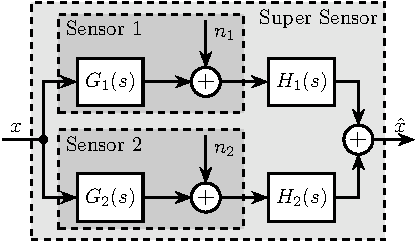
\includegraphics[scale=1.8]{figs/fusion_super_sensor.pdf}
\end{tikzfigure}

\begin{tikzfigure}[Sensor fusion architecture with sensor dynamics uncertainty]
  \label{fig:sensor_fusion_dynamic_uncertainty}
  \centering
  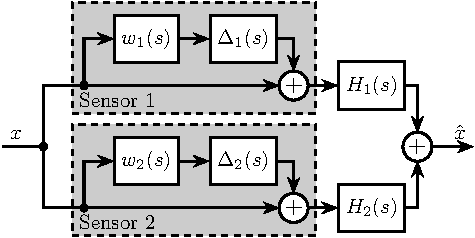
\includegraphics[scale=1.8]{figs/sensor_fusion_dynamic_uncertainty.pdf}
\end{tikzfigure}

\begin{tikzfigure}[Uncertainty set of the super sensor dynamics]
  \label{fig:uncertainty_set_super_sensor}
  \centering
  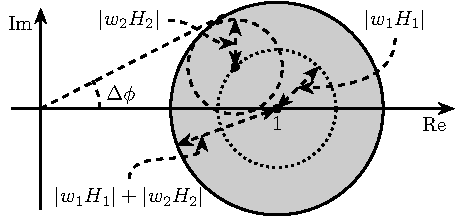
\includegraphics[scale=1.8]{figs/uncertainty_set_super_sensor.pdf}
\end{tikzfigure}}

\column{0.5}
\block[]{Complementary Filters Shaping using $\mathcal{H}_\infty$ Synthesis}{\begin{minipage}[t]{.6\linewidth}
  The \textbf{synthesis objective} is to \textbf{shape the norm of two filters}
  while ensuring their \textbf{complementary property}.
  This is equivalent to the conditions on the right where \(H_1(s)\) and
  \(H_2(s)\) are stable transfer function.
  $W_1(s)$ and $W_2(s)$ are \textbf{weighting functions} that are used to define
  wanted \textbf{upper bound of the complementary filter norms}.
  They should be \textbf{proper}, \textbf{stable} and \textbf{minimum phase}
  transfer functions.
\end{minipage}\hfill%
\begin{minipage}[t]{.38\linewidth}
  \vspace{-1em}
  \[ \tcmbox{\begin{align*}
       &H_1(s) + H_2(s) = 1 \\
       &|H_1(j\omega)| \le \frac{1}{|W_1(j\omega)|} \quad \forall\omega \\
       &|H_2(j\omega)| \le \frac{1}{|W_2(j\omega)|} \quad \forall\omega
     \end{align*}} \]
\end{minipage}

\bigskip

% \begin{equation*}
%   \begin{bmatrix} z_1 \\ z_2 \\ v \end{bmatrix} = P(s) \begin{bmatrix} w\\u \end{bmatrix}; \quad P(s) = \begin{bmatrix}W_1(s) & -W_1(s) \\ 0 & W_2(s) \\  1 & 0 \end{bmatrix}
% \end{equation*}

% The \(\mathcal{H}_\infty\) filter design problem is then to find a stable filter \(H_2(s)\) which based on \(v\), generates a signal \(u\) such that the \(\mathcal{H}_\infty\) norm from \(w\) to \([z_1, \ z_2]\) is less than one:
% \begin{equation*}
%   \begin{Vmatrix} \left[1 - H_2(s)\right] W_1(s) \\ H_2(s) W_2(s) \end{Vmatrix}_\infty \le 1
% \end{equation*}

% By defining \(H_1(s)\) as the complementary filter of \(H_2(s)\), we have:
% \begin{equation*}
%   \begin{Vmatrix} H_1(s) W_1(s) \\ H_2(s) W_2(s) \end{Vmatrix}_\infty \le 1
% \end{equation*}

% \begin{equation*}
%   H_1(s) \triangleq 1 - H_2(s)
% \end{equation*}

% Find $H_2(s)$ such that:
% \begin{gather*}
%   \begin{Vmatrix} \left[1 - H_2(s)\right] W_1(s) \\ H_2(s) W_2(s) \end{Vmatrix}_\infty \le 1 \\
%   H_1(s) \triangleq 1 - H_2(s)
% \end{gather*}

\bigskip

% Consider the architecture shown in Fig.~\ref{fig:h_infinity_robust_fusion} where
% $P(s)$ represents a \csquotes{generalized plant} containing the weights.

\begin{minipage}[t]{0.47\linewidth}
  This optimization problem is written as a \textbf{standard} \(\mathcal{H}_\infty\)
  \textbf{problem} (Fig.~\ref{fig:h_infinity_robust_fusion}).

  The \(\mathcal{H}_\infty\) synthesis applied to \(P(s)\) generates
  a stable filter \(H_2(s)\) such that the \(\mathcal{H}_\infty\) norm from \(w\) to \([z_1, \ z_2]\)
  is less than one.
  By defining \(H_1(s) \triangleq 1 - H_2(s)\), this is equivalent to the
  synthesis objective described above.
  \begin{tikzfigure}[$\mathcal{H}_\infty$ synthesis of
    complementary filters]
    \label{fig:h_infinity_robust_fusion}
    \centering
    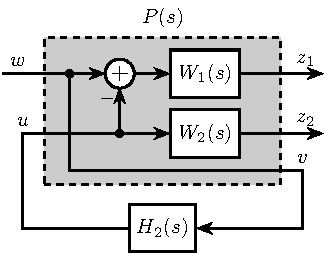
\includegraphics[scale=1.8]{figs/h_infinity_robust_fusion.pdf}
  \end{tikzfigure}
\end{minipage}\hfill
\begin{minipage}[t]{0.49\linewidth}
  This \(\mathcal{H}_\infty\) synthesis is first applied for the design of simple complementary
  filters (Fig.~\ref{fig:hinf_synthesis_results}).

  \begin{tikzfigure}[Frequency response of the weighting functions and
    complementary filters obtained using $\mathcal{H}_\infty$ synthesis]
    \label{fig:hinf_synthesis_results}
    \centering
    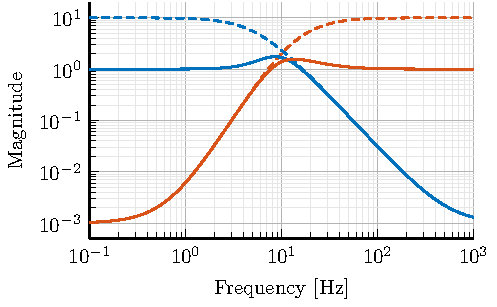
\includegraphics[width=\linewidth]{figs/hinf_synthesis_results.pdf}
  \end{tikzfigure}
\end{minipage}

% \textbf{Weighting Function Design}

% \begin{minipage}[t]{0.49\linewidth}
%   \begin{equation*}
%     W(s) = \left( \frac{
%         \hfill{} \frac{1}{\omega_0} \sqrt{\frac{1 - \left(\frac{G_0}{G_c}\right)^{\frac{2}{n}}}{1 - \left(\frac{G_c}{G_\infty}\right)^{\frac{2}{n}}}} s + \left(\frac{G_0}{G_c}\right)^{\frac{1}{n}}
%       }{
%         \left(\frac{1}{G_\infty}\right)^{\frac{1}{n}} \frac{1}{\omega_0} \sqrt{\frac{1 - \left(\frac{G_0}{G_c}\right)^{\frac{2}{n}}}{1 - \left(\frac{G_c}{G_\infty}\right)^{\frac{2}{n}}}} s + \left(\frac{1}{G_c}\right)^{\frac{1}{n}}
%       }\right)^n
%   \end{equation*}
% \end{minipage}\hfill
% \begin{minipage}[t]{0.49\linewidth}
%   \begin{tikzfigure}[Magnitude of a weighting function generated using the proposed formula \eqref{eq:weight_formula}, $G_0 = 1e^{-3}$, $G_\infty = 10$, $\omega_c = \SI{10}{Hz}$, $G_c = 2$, $n = 3$]
%     \label{fig:weight_formula}
%     \centering
%     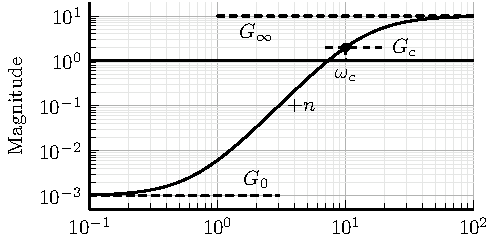
\includegraphics[width=\linewidth]{figs/weight_formula.pdf}
%   \end{tikzfigure}
% \end{minipage}

% \textbf{Three Complementary Filters}

% \begin{minipage}[t]{0.49\linewidth}
%   \begin{tikzfigure}[Architecture for $\mathcal{H}_\infty$ synthesis of three complementary filters]
%     \label{fig:comp_filter_three_hinf}
%     \centering
%     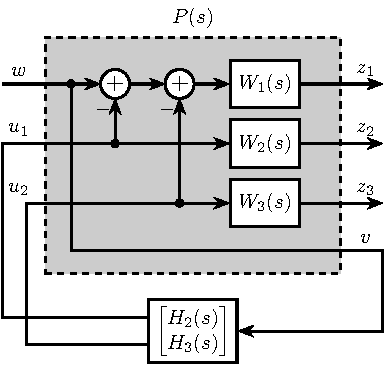
\includegraphics[scale=1.8]{figs/comp_filter_three_hinf.pdf}
%   \end{tikzfigure}
% \end{minipage}\hfill
% \begin{minipage}[t]{0.49\linewidth}
%   \begin{tikzfigure}[Frequency response of the weighting functions and three complementary filters obtained using $\mathcal{H}_\infty$ synthesis]
%     \label{fig:hinf_three_synthesis_results}
%     \centering
%     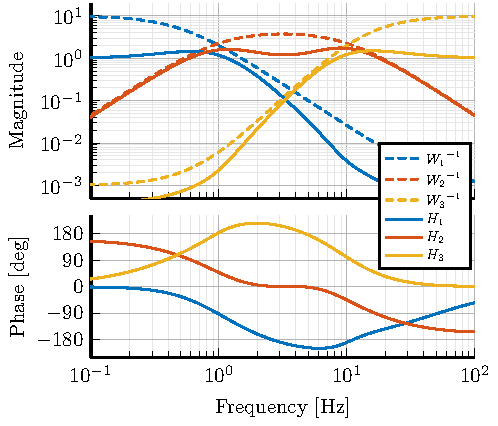
\includegraphics[scale=1.8]{figs/hinf_three_synthesis_results.pdf}
%   \end{tikzfigure}
% \end{minipage}

%%% Local Variables:
%%% TeX-master: "poster"
%%% End:}
\block[]{Design of Complementary Filters used in the Active Vibration Isolation System at the LIGO}{%%% Local Variables:
%%% TeX-master: "poster"
%%% End:

\textbf{Control Configuration}

\begin{minipage}[t]{0.49\linewidth}
  \begin{tikzfigure}[Specifications and weighting functions magnitude used for $\mathcal{H}_\infty$ synthesis]
    \label{fig:ligo_weights}
    \centering
    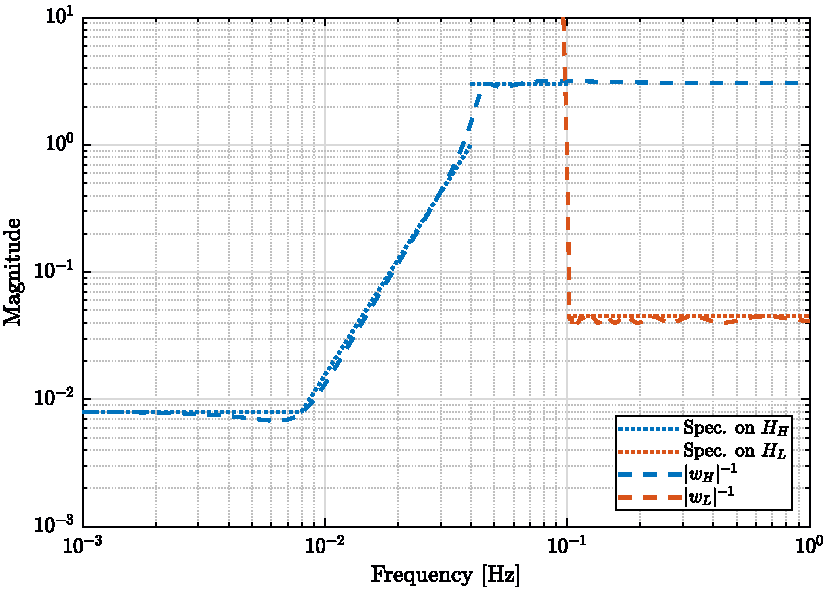
\includegraphics[width=\linewidth]{figs/ligo_weights.pdf}
  \end{tikzfigure}
\end{minipage}\hfill
\begin{minipage}[t]{0.49\linewidth}
  \begin{tikzfigure}[Comparison of the FIR filters (solid) designed in \cite{hua05_low_ligo} with the filters obtained with $\mathcal{H}_\infty$ synthesis (dashed)]
    \label{fig:comp_fir_ligo_hinf}
    \centering
    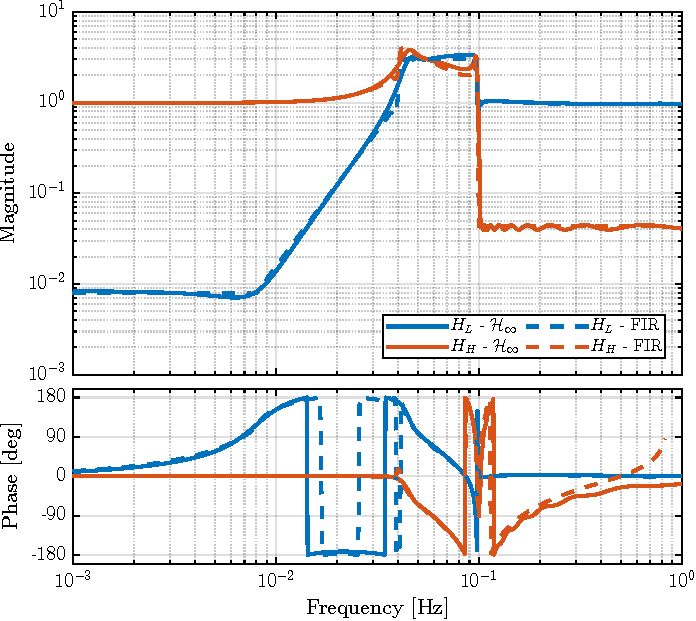
\includegraphics[width=\linewidth]{figs/comp_fir_ligo_hinf.pdf}
  \end{tikzfigure}
\end{minipage}
}
\block[]{Conclusion}{%%% Local Variables:
%%% TeX-master: "poster"
%%% End:

Complementary filters can be used to \textbf{combine multiple sensors} in order
to obtain a \textbf{super sensor}.
Specification on the \textbf{super sensor noise} and on the \textbf{robustness
  of the sensor fusion} are linked to the \textbf{norm of the complementary filters}.
A synthesis method that permits the \textbf{shaping of the complementary filters
  norms} has been proposed and has been successfully applied for the design of
complex filters.
}
\end{columns}

\begin{columns}
  \column{0.8}
  \block[]{}{%%% Local Variables:
%%% TeX-master: "poster"
%%% End:

\begin{minipage}[t]{0.1\linewidth}
  \textbf{Reference}
\end{minipage}\hfill
\begin{minipage}[t]{0.89\linewidth}
  \printbibliography[heading=none]
\end{minipage}

% \begin{minipage}[t]{0.2\linewidth}
%   \textbf{Acknowledgments}
% \end{minipage}\hfill
% \begin{minipage}[t]{0.8\linewidth}
%   This research benefited from a FRIA grant from the French Community of Belgium.
% \end{minipage}
}
  \column{0.2}
  \block[]{}{\textbf{Acknowledgments}

\bigskip

This research benefited from a FRIA grant from the French Community of Belgium.

\vspace{0.4em}

%%% Local Variables:
%%% mode: latex
%%% TeX-master: "poster"
%%% End:
}
\end{columns}

\end{document}